\documentclass[final,9pt,fleqn]{beamer}\usepackage[]{graphicx}\usepackage[]{xcolor}
% maxwidth is the original width if it is less than linewidth
% otherwise use linewidth (to make sure the graphics do not exceed the margin)
\makeatletter
\def\maxwidth{ %
  \ifdim\Gin@nat@width>\linewidth
    \linewidth
  \else
    \Gin@nat@width
  \fi
}
\makeatother

\definecolor{fgcolor}{rgb}{0.345, 0.345, 0.345}
\newcommand{\hlnum}[1]{\textcolor[rgb]{0.686,0.059,0.569}{#1}}%
\newcommand{\hlstr}[1]{\textcolor[rgb]{0.192,0.494,0.8}{#1}}%
\newcommand{\hlcom}[1]{\textcolor[rgb]{0.678,0.584,0.686}{\textit{#1}}}%
\newcommand{\hlopt}[1]{\textcolor[rgb]{0,0,0}{#1}}%
\newcommand{\hlstd}[1]{\textcolor[rgb]{0.345,0.345,0.345}{#1}}%
\newcommand{\hlkwa}[1]{\textcolor[rgb]{0.161,0.373,0.58}{\textbf{#1}}}%
\newcommand{\hlkwb}[1]{\textcolor[rgb]{0.69,0.353,0.396}{#1}}%
\newcommand{\hlkwc}[1]{\textcolor[rgb]{0.333,0.667,0.333}{#1}}%
\newcommand{\hlkwd}[1]{\textcolor[rgb]{0.737,0.353,0.396}{\textbf{#1}}}%
\let\hlipl\hlkwb

\usepackage{framed}
\makeatletter
\newenvironment{kframe}{%
 \def\at@end@of@kframe{}%
 \ifinner\ifhmode%
  \def\at@end@of@kframe{\end{minipage}}%
  \begin{minipage}{\columnwidth}%
 \fi\fi%
 \def\FrameCommand##1{\hskip\@totalleftmargin \hskip-\fboxsep
 \colorbox{shadecolor}{##1}\hskip-\fboxsep
     % There is no \\@totalrightmargin, so:
     \hskip-\linewidth \hskip-\@totalleftmargin \hskip\columnwidth}%
 \MakeFramed {\advance\hsize-\width
   \@totalleftmargin\z@ \linewidth\hsize
   \@setminipage}}%
 {\par\unskip\endMakeFramed%
 \at@end@of@kframe}
\makeatother

\definecolor{shadecolor}{rgb}{.97, .97, .97}
\definecolor{messagecolor}{rgb}{0, 0, 0}
\definecolor{warningcolor}{rgb}{1, 0, 1}
\definecolor{errorcolor}{rgb}{1, 0, 0}
\newenvironment{knitrout}{}{} % an empty environment to be redefined in TeX

\usepackage{alltt}
\setbeamertemplate{bibliography item}[text]
\setbeamertemplate{caption}[numbered]
\usepackage{url,lmodern}
\usepackage{amsmath,amsfonts,amssymb,graphicx,
  amsthm,subfigure,multirow,hyperref,textcomp,natbib}
\usepackage[iso,american]{isodate}
\usepackage{listings}
\usepackage[dvipsnames]{xcolor}
\hypersetup{colorlinks=true,urlcolor=BrickRed,linkcolor=BrickRed}

\definecolor{mygray}{gray}{0.3}
\setbeamertemplate{itemize item}{\color{mygray}$\blacktriangleright$}
\addtobeamertemplate{frametitle}{\vskip 0.4in}{}

\usepackage{eso-pic}
\setlength{\paperwidth}{16.5in}
\setlength{\paperheight}{10.5in}
\setlength{\mathindent}{5pt}
\usepackage{lmodern}
\setbeamertemplate{navigation symbols}{}

\defbeamertemplate*{footline}{infolines theme} { \leavevmode%
  \hbox{%
    \begin{beamercolorbox}[wd=.333333\paperwidth,ht=2.25ex,dp=1ex,center]{author
        in head/foot}%
      \usebeamerfont{author in
        head/foot}\insertshortauthor%~~(\insertshortinstitute)
    \end{beamercolorbox}%
    \begin{beamercolorbox}[wd=.333333\paperwidth,ht=2.25ex,dp=1ex,center]{title
        in head/foot}%
      \usebeamerfont{title in head/foot}\insertshorttitle
    \end{beamercolorbox}%
    \begin{beamercolorbox}[wd=.333333\paperwidth,ht=2.25ex,dp=1ex,right]{date
        in head/foot}%
      \usebeamerfont{date in head/foot}\insertshortdate{}\hspace*{2em}
      \insertframenumber{} / \inserttotalframenumber\hspace*{2ex}
    \end{beamercolorbox}}%
  \vskip0pt%
}
\newcommand\AtPagemyUpperLeft[1]{\AtPageLowerLeft{%
    \put(\LenToUnit{0.88\paperwidth},\LenToUnit{0.88\paperheight}){#1}}}
\AddToShipoutPictureFG{
  \AtPagemyUpperLeft{{
      \href{http://mc-stan.org/}{\includegraphics[scale=0.25,keepaspectratio]{../logos/Stan.png}}
      \hspace{0.025in}
      \href{http://ggplot2.tidyverse.org}{\includegraphics[scale=0.5,keepaspectratio]{../logos/ggplot2.png}}
}}
}%


\setbeamertemplate{footline}{\hfill {\footnotesize \href{https://creativecommons.org/licenses/by-sa/4.0/}{CC BY-SA 4.0} $\circ$ Nicholas J. Clark $\circ$ Learn more at \href{https://nicholasjclark.github.io/mvgam/index.html}{https://nicholasjclark.github.io/mvgam/index.html} $\circ$ package version $1.0.9$ $\circ$ updated: \today} \hspace {0.1in} \vspace{0.1in}}
\IfFileExists{upquote.sty}{\usepackage{upquote}}{}
\begin{document}









\begin{frame}[fragile]
  \frametitle{{\fontsize{41}{43} \selectfont \textcolor{mygray}{mvgam ::}} {\fontsize{25}{25} \textbf{\textcolor{mygray}{CHEATSHEET}}}}
\vspace{-0.6in}
  \begin{columns}
    \begin{column}{0.02\paperwidth} % left margin space
    \end{column}

    \begin{column}{0.3\paperwidth}

\begin{block}
\noindent\makebox[\linewidth]{\rule{0.3\paperwidth}{0.2pt}}

The \texttt{mvgam} package provides tools for fitting and interrogating univariate or multivariate time series models that can include nonlinear smooth functions of covariates, dynamic temporal processes and random effects. A wide variety of latent dynamic processes can be specified. The package also provides tools for interpreting effects, computing and scoring forecasts, as well as generating model code and data objects for further customisation. Models are fitted using \texttt{Stan} for full Bayesian inference.

\end{block}

\begin{block}{{\fontsize{21}{21} \selectfont \color{BrickRed} Modelling with \texttt{\color{Orchid} mvgam()}}}
Usage: \texttt{\color{Orchid} mvgam(formula, trend\_formula, data, trend\_model, family, ...)}

\medskip
\texttt{\color{Orchid} formula}: observation model regression formula, built off the \texttt{mgcv} package. See \texttt{\color{Orchid}?mvgam\_formulae} for more guidance

\medskip
\texttt{\color{Orchid} trend\_formula}: optional process model formula (see \href{https://nicholasjclark.github.io/mvgam/articles/trend_formulas.html}{the State-Space model vignette} and \href{https://nicholasjclark.github.io/mvgam/articles/trend_formulas.html}{the shared latent states vignette} for guidance on using trend formulae)

\medskip
\texttt{\color{Orchid} data}: a \texttt{data.frame} or \texttt{list} containing the response variable(s) and optional predictor variables. See \href{https://nicholasjclark.github.io/mvgam/articles/data_in_mvgam.html}{the data formatting vignette} for guidance on data preparation

\medskip
\texttt{\color{Orchid} trend\_model}: optional latent dynamic process. Options include:
\begin{itemize}

\item\texttt{\color{Orchid} None}: default, no dynamic trend

\item\texttt{\color{Orchid} RW(ma = FALSE, cor = FALSE)}: random walk

\item\texttt{\color{Orchid} AR(p = 1, ma = FALSE, cor = FALSE)}: autoregressive

\item\texttt{\color{Orchid} VAR(ma = FALSE, cor = FALSE)}: vector autoregressive

\item\texttt{\color{Orchid} PW(growth = 'linear')}: piecewise linear

\item\texttt{\color{Orchid} PW(growth = 'logistic')}: piecewise logistic, with max saturation

\item\texttt{\color{Orchid} GP()}: squared exponential Gaussian Process
\end{itemize}
For autoregressive processes (\texttt{\color{Orchid} RW(), AR() or VAR()}), moving average and correlated process errors can also be specified by changing the \texttt{\color{Orchid} ma} and \texttt{\color{Orchid} cor} arguments

\medskip
\texttt{\color{Orchid} family}: observation distribution. Options include (among others):
\begin{itemize}

\item\texttt{\color{Orchid} gaussian()}: Gaussian with identity link

\item\texttt{\color{Orchid} student-t()}: Student's T with identity link

\item\texttt{\color{Orchid} lognormal()}: LogNormal with identity link

\item\texttt{\color{Orchid} Gamma()}: Gamma with log link

\item\texttt{\color{Orchid} betar()}: Beta with logit link

\item\texttt{\color{Orchid} poisson()}: Poisson with log link

\item\texttt{\color{Orchid} nb()}: Negative Binomial with log link
\end{itemize}

\medskip
See \href{https://nicholasjclark.github.io/mvgam/articles/mvgam_overview.html}{the introductory vignette} for more guidance on supported families and dynamic processes

\medskip
\texttt{\color{Orchid} ...}: other arguments such as user-specified \texttt{\color{Orchid} priors}, \texttt{\color{Orchid} newdata} for generating probabilistic forecasts and options to control \texttt{\color{Orchid} Stan} MCMC parameters

\medskip
\textbf{\color{BrickRed} Prior to modelling}, it is useful to:
\begin{itemize}

\item Inspect features of the data with \texttt{\color{Orchid} plot\_mvgam\_series()}

\item Ensure there are no \texttt{\color{Orchid} NA}'s in predictors (though \texttt{\color{Orchid} NA}'s are allowed in response variables). See \href{https://nicholasjclark.github.io/mvgam/articles/data_in_mvgam.html}{the data formatting vignette} for guidance on data preparation

\item Inspect default priors with \texttt{\color{Orchid} get\_mvgam\_priors()}

\item Make any necessary changes to default priors with \texttt{\color{Orchid} prior()}

\end{itemize}

\medskip
\texttt{\color{Orchid} sim\_mvgam()} is useful to generate simple example datasets
\begin{knitrout}
\definecolor{shadecolor}{rgb}{0.969, 0.969, 0.969}\color{fgcolor}\begin{kframe}
\begin{alltt}
\hlstd{simdat} \hlkwb{<-} \hlkwd{sim_mvgam}\hlstd{(}\hlkwc{n_series} \hlstd{=} \hlnum{1}\hlstd{)}
\hlstd{model} \hlkwb{<-} \hlkwd{mvgam}\hlstd{(}\hlkwc{formula} \hlstd{= y} \hlopt{~} \hlkwd{s}\hlstd{(season,} \hlkwc{bs} \hlstd{=} \hlstr{'cc'}\hlstd{),}
               \hlkwc{trend_model} \hlstd{=} \hlkwd{RW}\hlstd{(),} \hlkwc{data} \hlstd{= simdat}\hlopt{$}\hlstd{data_train)}
\end{alltt}
\end{kframe}
\end{knitrout}

Use \texttt{\color{Orchid} code(model)} to see the auto-generated \texttt{Stan} code

\end{block}
\end{column}


\begin{column}{.03\paperwidth}
\end{column}


\begin{column}{0.3\paperwidth}
\vspace{0.52in}
\noindent\makebox[\linewidth]{\rule{0.3\paperwidth}{0.2pt}}
\begin{block}{{\fontsize{21}{21} \selectfont \color{BrickRed} Diagnostics and Inference}}

\smallskip
{{\fontsize{11}{11} \selectfont \color{mygray} What effects has the model estimated?}}

\medskip
\texttt{\color{Orchid} summary(model)} and \texttt{\color{Orchid} coef(model)}: posterior summaries and diagnostics

\medskip
\texttt{\color{Orchid} fitted(model)}, \texttt{\color{Orchid} logLik(model)} and \texttt{\color{Orchid} residuals(model)}: posterior expectations, pointwise Log-Likelihoods and randomized quantile residuals

\medskip
\texttt{\color{Orchid} loo(model)} and \texttt{\color{Orchid} loo\_compare(model1, model2, ...)}: calculate approximate leave-one-out information criteria

\medskip
\texttt{\color{Orchid} mcmc\_plot(model)}: visualize posterior summaries, pairs plots and a wide range of MCMC diagnostics using functionality from the \texttt{Bayesplot} package

\begin{knitrout}
\definecolor{shadecolor}{rgb}{0.969, 0.969, 0.969}\color{fgcolor}

{\centering 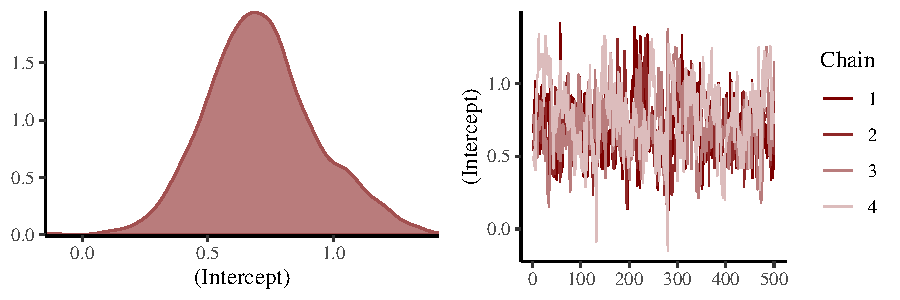
\includegraphics[width=\maxwidth]{figure/unnamed-chunk-4-1} 

}


\end{knitrout}

\medskip
Use \texttt{\color{Orchid} as.data.frame(model)}, \texttt{\color{Orchid} as.matrix(model)}, or \texttt{\color{Orchid} as.array(model)} for posterior extraction. Use \texttt{\color{Orchid} variables(model)} to determine what parameters are available for extraction

\medskip
The \texttt{S3} \texttt{\color{Orchid} plot()} function applied to models can visualise smooth functions (\texttt{\color{Orchid} type = 'smooths'}), random effects (\texttt{\color{Orchid} type = 're'}), posterior predictions and trend estimates (\texttt{\color{Orchid} type = 'forecast'} or \texttt{\color{Orchid} type = 'trend'}) uncertainty contributions (\texttt{\color{Orchid} type = 'uncertainty'}) or randomized quantile residual diagnostics (\texttt{\color{Orchid} type = 'residuals'}). Use \texttt{\color{Orchid} trend\_effects = TRUE} to visualise effects from any process model formulae

\medskip
\texttt{\color{Orchid} conditional\_effects(model)} gives useful conditional effect plots on either the response or the link scale

\smallskip
\begin{knitrout}
\definecolor{shadecolor}{rgb}{0.969, 0.969, 0.969}\color{fgcolor}

{\centering 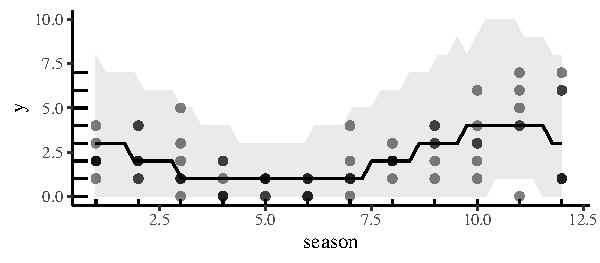
\includegraphics[width=\maxwidth]{figure/unnamed-chunk-5-1} 

}


\end{knitrout}

For most \texttt{mvgam} models, functions from the \texttt{marginaleffects} package can be used for more targeted prediction-based inference. See \href{https://marginaleffects.com/}{The Marginal Effects Zoo} for guidance on computing and plotting predictions, slopes and comparisons
\begin{knitrout}
\definecolor{shadecolor}{rgb}{0.969, 0.969, 0.969}\color{fgcolor}

{\centering 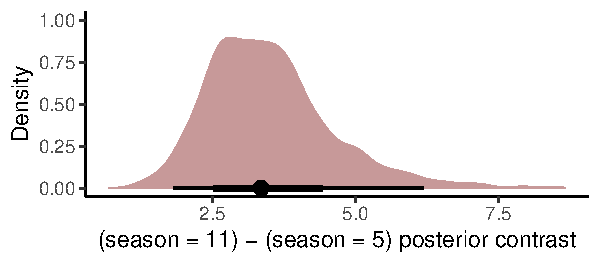
\includegraphics[width=\maxwidth]{figure/unnamed-chunk-6-1} 

}


\end{knitrout}

\end{block}
\end{column}


\begin{column}{.03\paperwidth}
\end{column}


\begin{column}{0.3\paperwidth}
\vspace{0.37in}
\noindent\makebox[\linewidth]{\rule{0.3\paperwidth}{0.2pt}}
\begin{block}{{\fontsize{21}{21} \selectfont \color{BrickRed} Prediction and forecasting}}

\smallskip
{{\fontsize{11}{11} \selectfont \color{mygray} How good are model predictions?}}

\medskip
Use \texttt{\color{Orchid} predict(model)} with \texttt{\color{Orchid} newdata} to make predictions for inference purposes. Change the \texttt{\color{Orchid} type} argument for different types of predictions (link scale, expectation or response scale). Or use the \texttt{brms} package equivalents \texttt{\color{Orchid} posterior\_predict(model)}, \texttt{\color{Orchid} posterior\_linpred(model)} or \texttt{\color{Orchid} posterior\_epred(model)}. If generating forecasts for future timepoints, use the \texttt{\color{Orchid} forecast()} function (see below)

\medskip
Use \texttt{\color{Orchid} ppc(model)} to plot various kinds of posterior predictive checks to compare model predictions against true observations

\medskip
Extract in-sample posterior predictions with \texttt{\color{Orchid} hindcast(model)}. If validation data exist, generate forecast predictions with \texttt{\color{Orchid} forecast(model, newdata = newdata)}. As above, change the \texttt{\color{Orchid} type} argument for predictions on different scales. Both functions generate an object of class \texttt{mvgam\_forecast}, that can be plotted with an \texttt{S3} \texttt{\color{Orchid} plot()} function. See \href{https://nicholasjclark.github.io/mvgam/articles/forecast_evaluation.html}{the forecasting vignette} for more details about how to produce forecasts.

\begin{knitrout}
\definecolor{shadecolor}{rgb}{0.969, 0.969, 0.969}\color{fgcolor}

{\centering 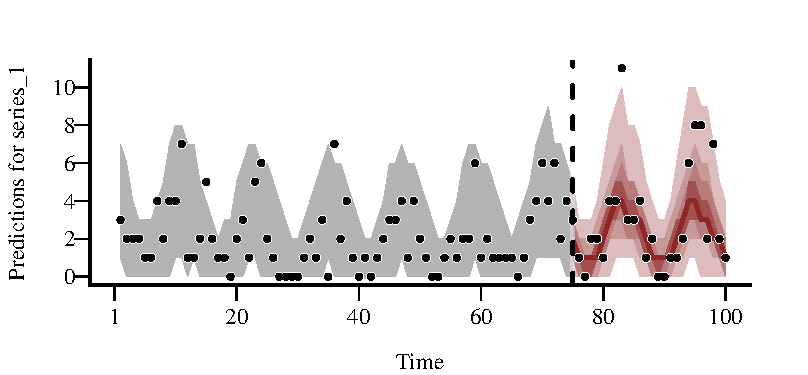
\includegraphics[width=\maxwidth]{figure/unnamed-chunk-7-1} 

}


\end{knitrout}

\smallskip
Compute probabilistic forecast scores using proper scoring rules with the \texttt{\color{Orchid} score()} function:
\begin{knitrout}
\definecolor{shadecolor}{rgb}{0.969, 0.969, 0.969}\color{fgcolor}\begin{kframe}
\begin{alltt}
\hlstd{fc} \hlkwb{<-} \hlkwd{forecast}\hlstd{(model,} \hlkwc{newdata} \hlstd{= simdat}\hlopt{$}\hlstd{data_test,} \hlkwc{type} \hlstd{=} \hlstr{'response'}\hlstd{)}
\hlstd{crps} \hlkwb{<-} \hlkwd{score}\hlstd{(fc,} \hlkwc{score} \hlstd{=} \hlstr{'crps'}\hlstd{)}
\hlstd{dplyr}\hlopt{::}\hlkwd{glimpse}\hlstd{(crps}\hlopt{$}\hlstd{series_1)}
\end{alltt}
\end{kframe}
\end{knitrout}

\begin{knitrout}
\definecolor{shadecolor}{rgb}{0.969, 0.969, 0.969}\color{fgcolor}\begin{kframe}
\begin{verbatim}
## Rows: 25
## Columns: 5
## $ score          <dbl> 0.2315, 0.3944, 0.7198, 0~
## $ in_interval    <dbl> 1, 1, 1, 1, 1, 1, 1, 0, 1~
## $ interval_width <dbl> 0.9, 0.9, 0.9, 0.9, 0.9, ~
## $ eval_horizon   <int> 1, 2, 3, 4, 5, 6, 7, 8, 9~
## $ score_type     <chr> "crps", "crps", "crps", "~
\end{verbatim}
\end{kframe}
\end{knitrout}
\smallskip
Available proper scoring rules in the \texttt{\color{Orchid} score()} function include:
\begin{itemize}

\item \texttt{\color{Orchid} type = 'crps'}: Continuous Rank Probability Score (univariate)
\item \texttt{\color{Orchid} type = 'drps'}: Discrete Rank Probability Score (univariate)
\item \texttt{\color{Orchid} type = 'elpd'}: Expected Log Predictive Density (univariate)
\item \texttt{\color{Orchid} type = 'sis'}: Scaled Interval Score (univariate)
\item \texttt{\color{Orchid} type = 'energy'}: Energy Score (multivariate)
\item \texttt{\color{Orchid} type = 'variogram'}: Variogram Score (multivariate)
\end{itemize}

\medskip
Use \texttt{\color{Orchid} lfo\_cv(model)} for approximate leave-future-out cross-validation with an expanding window training technique (see \href{https://www.tandfonline.com/doi/full/10.1080/00949655.2020.1783262}{Bürkner et al. 2020} for details of the algorithm). This generates expected log predictive density scores at user-specified forecast horizons, which can be used to compare different models

\end{block}
\end{column}

\end{columns}
\end{frame}

\end{document}
